\documentclass[11pt]{beamer}
\usepackage{helvet} %font
\beamertemplatenavigationsymbolsempty
\usetheme{JuanLesPins}
\usefonttheme{structurebold}

\usepackage[french]{babel}
\usepackage[utf8]{inputenc}
\usepackage[T1]{fontenc}
\usepackage{amssymb,amsmath}
\usepackage{tikz}
\usepackage{xcolor,colortbl}
\usetikzlibrary{arrows,positioning}
\usepackage{listings}
\usepackage{wasysym}

\newenvironment{slide}[1]{%
\begin{frame}[environment=slide]
\frametitle{#1~\hfill~
\includegraphics[height=1.2cm]{./epitech.png}}
}{%
\end{frame}
}
\setbeamercolor{structure}{fg=red}
\setbeamercolor{frametitle}{bg=black,fg=white}
\definecolor{gris}{gray}{0.6}
\definecolor{grisclair}{gray}{0.9}

\newtheorem{exercice}{Exercice}

\title{Big Data I : visualisation et traitement de données massives}
\author{}
\date{}

\newcommand{\Python}[1]{
	{\small	\lstinputlisting[language=Python]{./#1.py}}
}
\newenvironment{pyenvsmall}
	{ \ttfamily \tiny }
	{\par  }

\newcommand{\Pythonsmall}[1]{
	\begin{pyenvsmall}
		\vspace{-0.25cm}
		\lstinputlisting[language=Python]{./#1.py}
		\vspace{-0.3cm}
	\end{pyenvsmall}
}
\newcommand{\elimine}[1]{{\textcolor{lightgray}{#1}}}


\begin{document}


\begin{slide}{Ressources nécessaires}

Ce cours est entièrement conçu en \textbf{Python 3}. Si vous êtes habitués à R, vous pouvez avec quelques aménagements suivre ce cours en R ; pour tous les autres nous recommandons l'installation des logiciels suivants :

\vspace{0.2cm}

\begin{itemize}
	\item Python 3.x. Si vous n'êtes pas familiers avec l'installation de packages Python, choisissez la distribution Miniconda.
	\item l'IDE Pyzo. Configurez le shell pour utiliser Miniconda.
	\item les packages suivants (via l'IDE avec conda ou en utilisant pip) : NumPy, SciPy, matplotlib, pandas et sklearn
\end{itemize}

\end{slide}

\section*{Visualisation}

\subsection*{Motivation}

\begin{slide}{Des représentations naturelles ?}

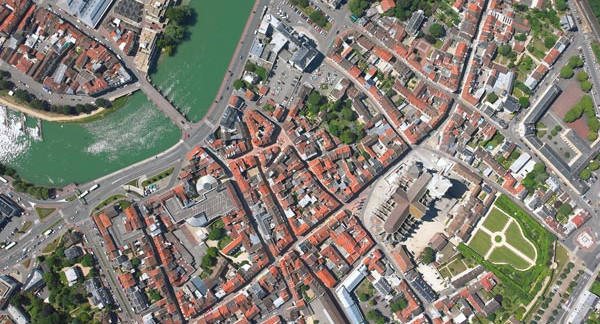
\includegraphics[scale=0.5]{meaux}


\end{slide}

\begin{slide}{Des représentations naturelles ?}
\begin{center}

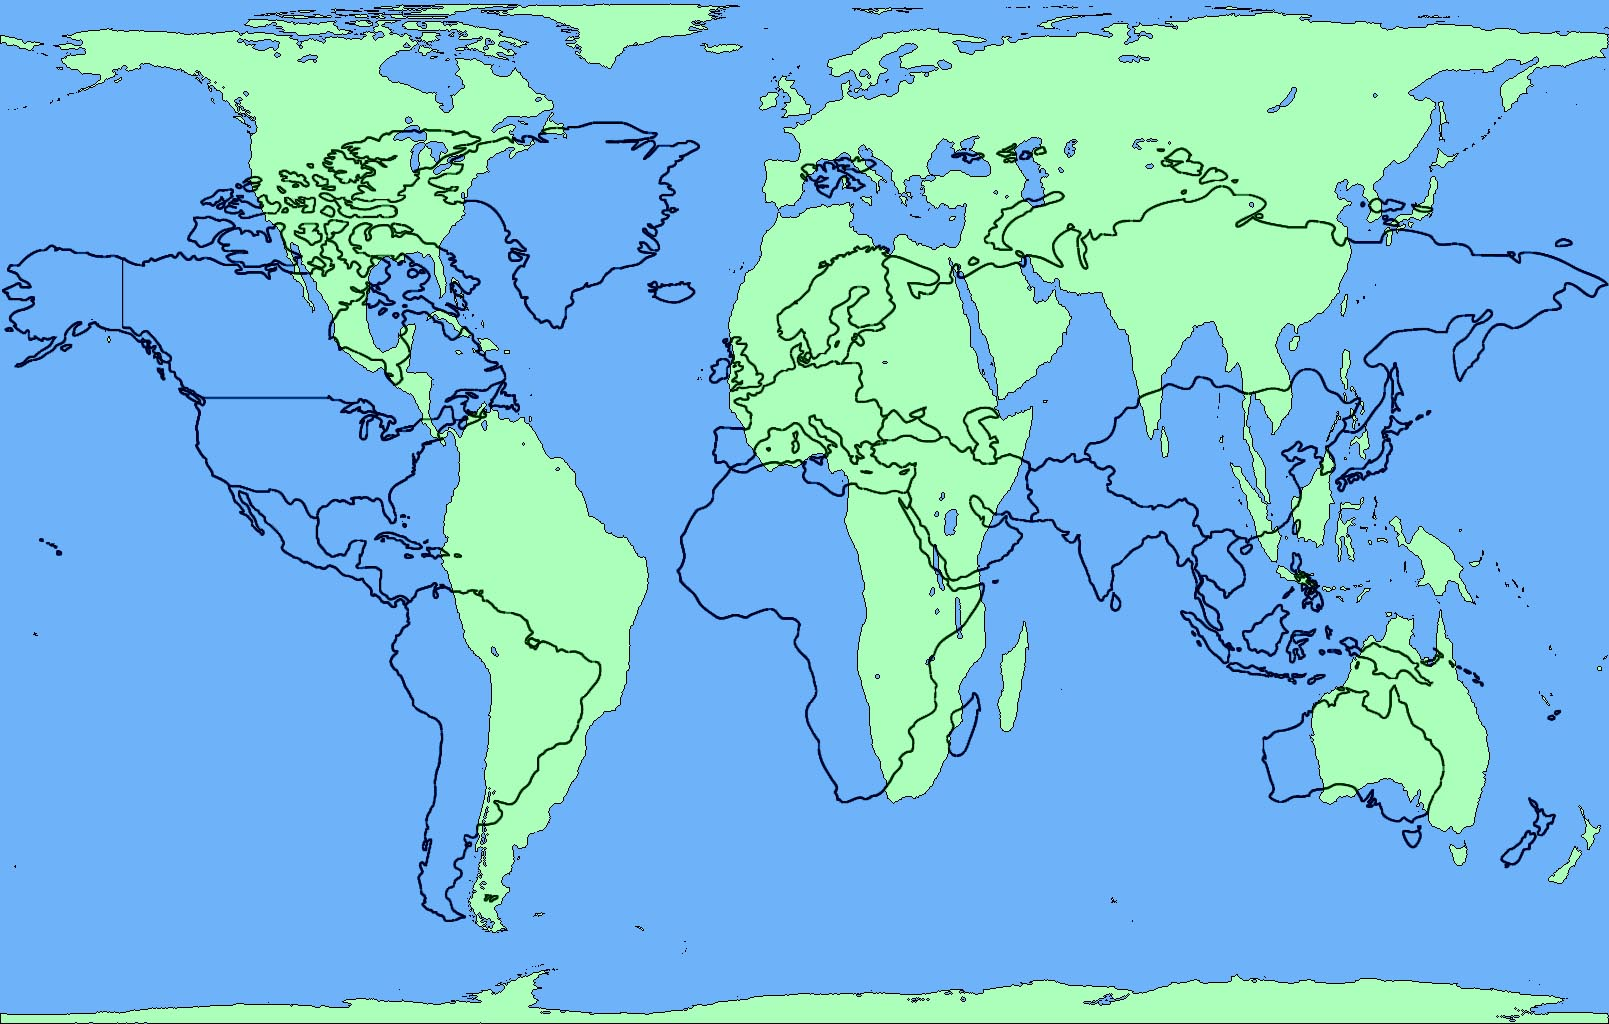
\includegraphics[scale=0.15]{projections}

\end{center}
\end{slide}

\begin{slide}{Des représentations naturelles ?}

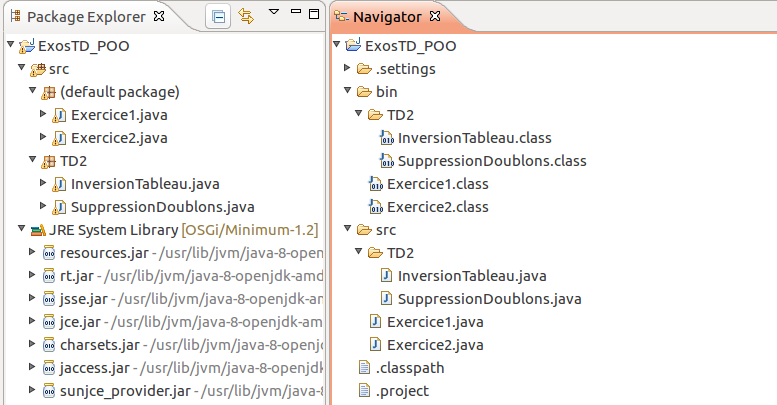
\includegraphics[scale=0.35]{files}

\end{slide}

\begin{slide}{Des représentations naturelles ?}

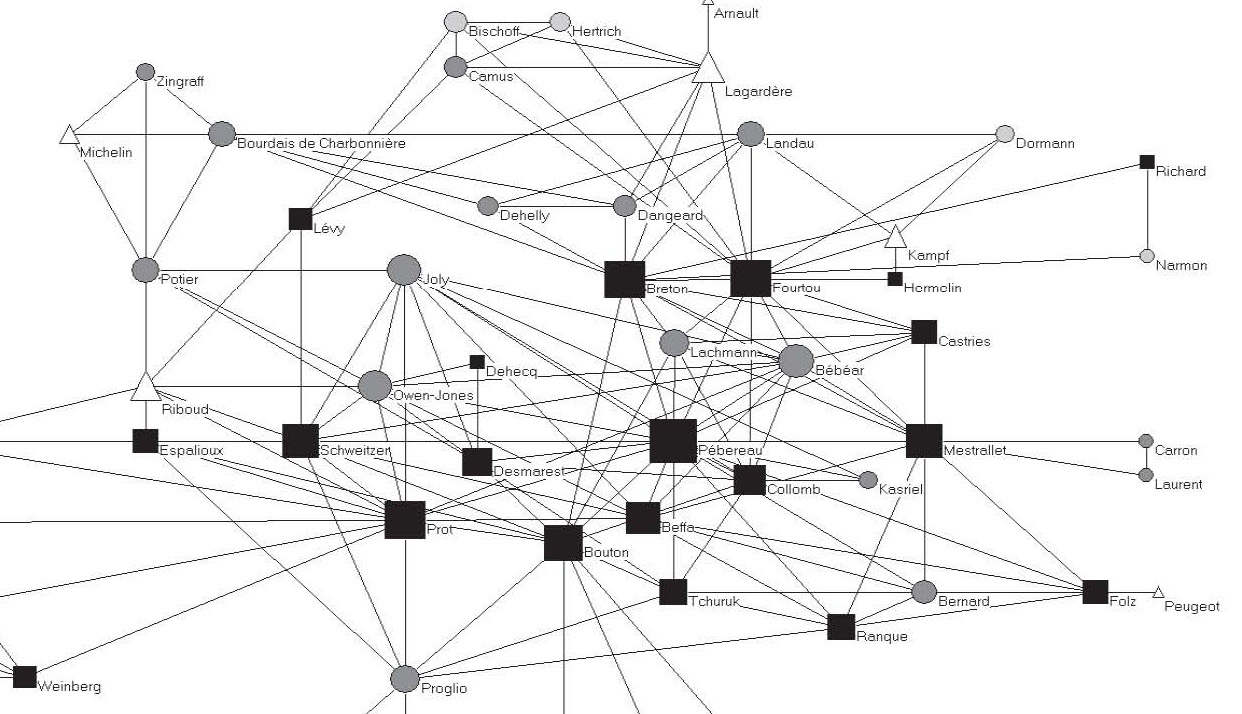
\includegraphics[scale=0.6]{dudouet}

\end{slide}

\begin{slide}{Problème: multidimensionnalité}

\begin{center}

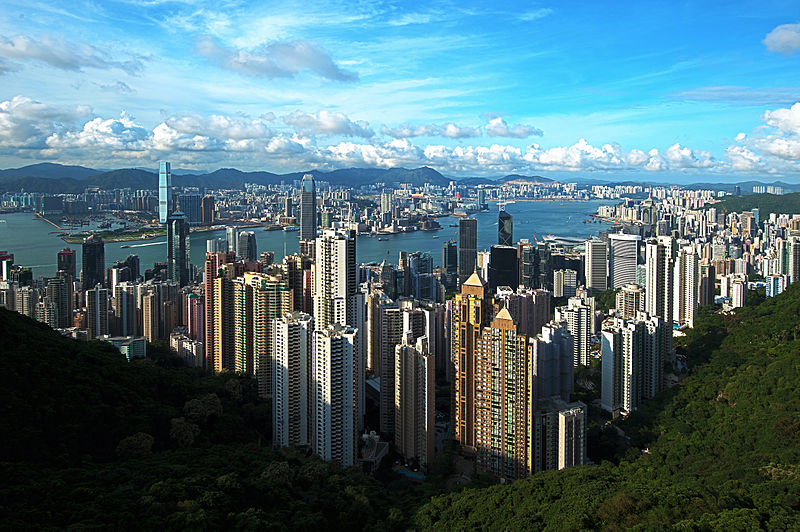
\includegraphics[scale=0.95]{hongkong}

\end{center}
\end{slide}

\begin{slide}{Problème: multidimensionnalité}

\begin{center}

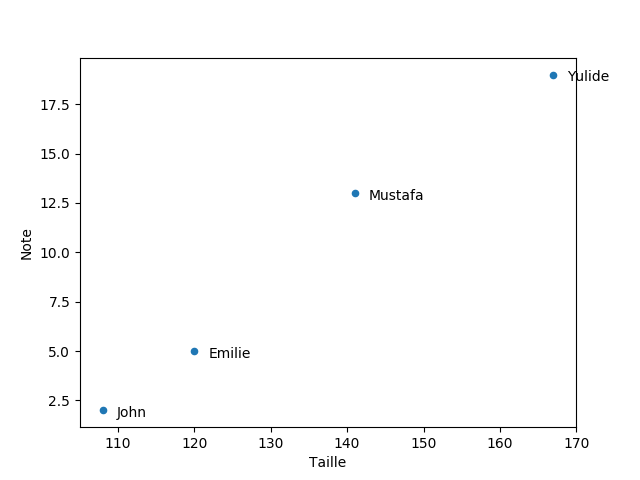
\includegraphics[scale=0.4]{plot1}

\end{center}
\end{slide}

\begin{slide}{Problème: multidimensionnalité}
\begin{center}
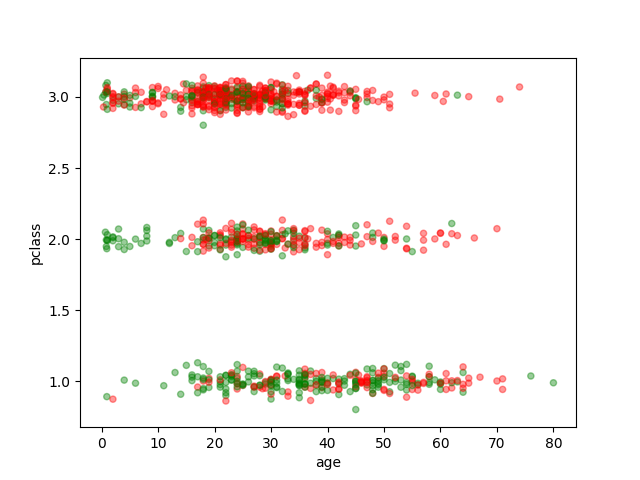
\includegraphics[scale=0.4]{titanic_plot}
\end{center}
\end{slide}

\begin{slide}{Problème: multidimensionnalité}
\begin{center}
{\tiny \input{data3.txt}}
\end{center}
\end{slide}

\begin{slide}{Problème: multidimensionnalité}
\begin{center}
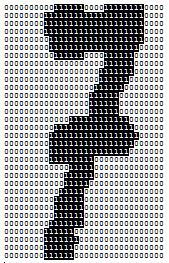
\includegraphics[scale=.75]{optdigits-7}
\end{center}
\end{slide}

\subsection*{Sélection de variables}

\begin{slide}{Scatter Matrix}
\begin{center}
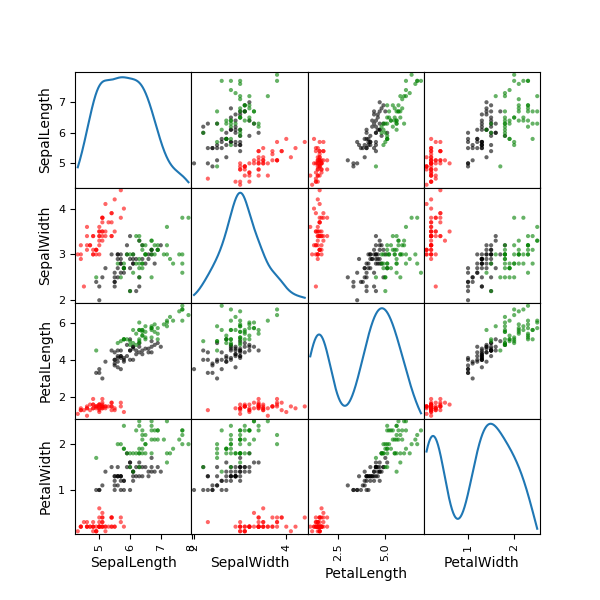
\includegraphics[scale=0.4]{iris_matrix}
\end{center}
\end{slide}


\begin{slide}{Scatter Matrix}
\begin{center}
\Python{scatter_matrix}
\end{center}
\end{slide}

\begin{slide}{Scatter Matrix}
\begin{center}
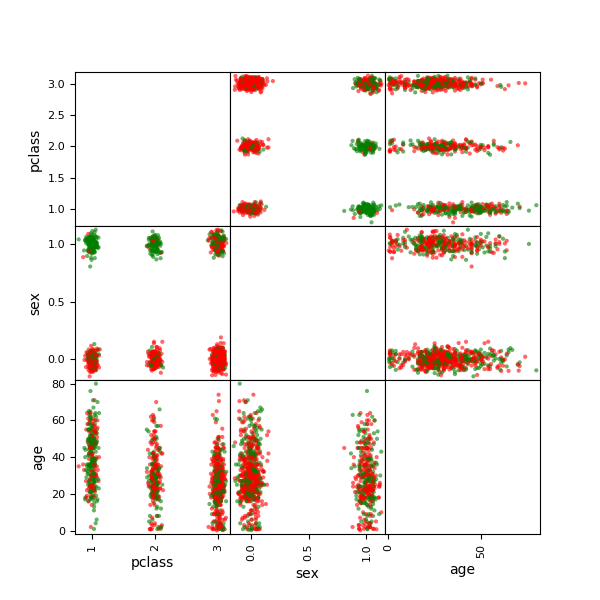
\includegraphics[scale=0.4]{titanic_matrix}
\end{center}
\end{slide}

\begin{slide}{ACP}
\begin{center}
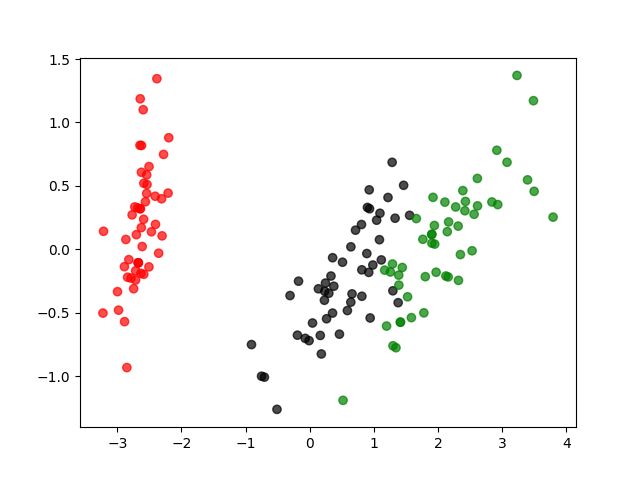
\includegraphics[scale=0.4]{iris_acp}
\end{center}
\end{slide}

\begin{slide}{ACP}
\begin{center}
\Python{acp}
\end{center}
\end{slide}

\begin{slide}{ACP}
\begin{center}
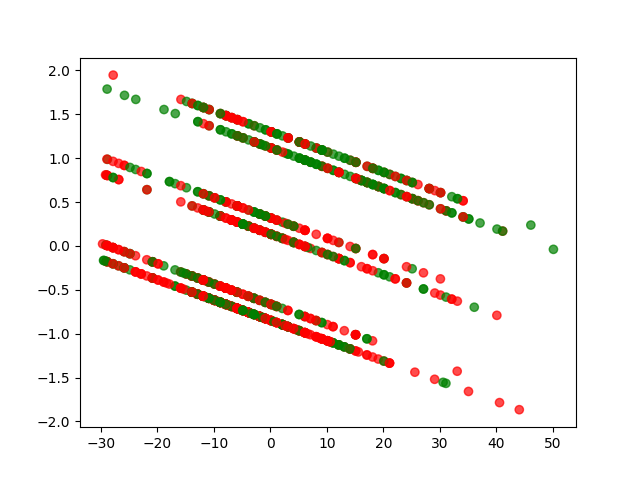
\includegraphics[scale=0.4]{titanic_acp}
\end{center}
\end{slide}

\begin{slide}{ACP}
\begin{center}
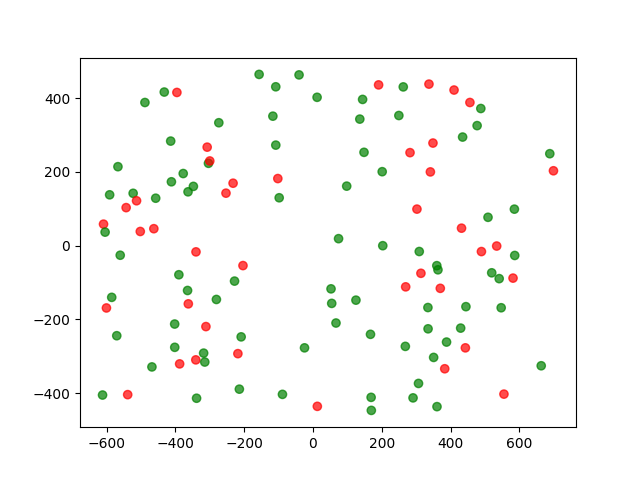
\includegraphics[scale=0.4]{titanic_acp_mv}
\end{center}
\end{slide}

\end{document}